
\chapter{Literature Review}
\label{chap:lit-review}


\ifpdf
    \graphicspath{{2_literature_review/figures/PNG/}{2_literature_review/figures/PDF/}{2_literature_review/figures/}}
\else
    \graphicspath{{2_literature_review/figures/EPS/}{2_literature_review/figures/}}
\fi

%: ----------------------- contents from here ------------------------


\section{Artificial Intelligence and Machine Learning}

Artificial Intelligence (AI) is a broad research field focused on designing and studying computational systems capable of performing tasks traditionally associated with human intelligence, such as reasoning, learning, problem-solving, perception, planning, and decision-making \cite{russell2021}.


 Rather than relying on a single methodology, AI involves all sorts of approaches that allow machines to perceive their environment and select actions that increase the probability of achieving defined objectives.

Since its formal recognition as an academic discipline in the mid-20th century, AI research has pursued objectives such as knowledge representation, logical reasoning, natural language understanding, visual perception, and autonomous control \cite{russell2021}. Achieving these objectives has required integrating diverse techniques, including symbolic logic, search and optimization methods, probabilistic modeling, artificial neural networks, and insights from related fields such as psychology, neuroscience, linguistics, and economics. Consequently, AI is best characterized as a multidisciplinary research area unified by the pursuit of intelligent behavior.

From the AI sphere, the Machine Learning (ML) has emerged as one of the most significant paradigms. Rather than relying on explicitly hand-crafted rules like GOFAI, machine learning focuses on algorithms that improve performance on specific tasks through experience, without human-defined if-else rules. This shift has been critical for solving problems that involve many variables, where manual rule specification is impractical. Advances in computing power and data availability have enabled learning-based approaches to consistently improve and, in many cases, surpass classical symbolic reasoning systems across diverse application domains.

Machine learning methods are typically classified into three categories, which are distinguished by the type of learning signals provided to the agent:

\begin{itemize}

  \item \textbf{Supervised Learning}, in which an algorithm learns a mapping from inputs to outputs using labeled data and optimizes a predefined loss function.

  \item \textbf{Unsupervised Learning}, where the objective is to discover latent structure in unlabeled data, such as clusters or low-dimensional representations.

  \item \textbf{Reinforcement Learning (RL)}, where an agent learns through direct interaction with an environment and receives only scalar reward signals as feedback.

\end{itemize}

Reinforcement learning differs fundamentally from supervised and unsupervised learning. RL is inherently interactive and sequential. The data distribution during training is not fixed; the agent's actions influence it. Each decision impacts immediate rewards, future states, and the data available for future learning. This feedback loop introduces challenges unique to RL, including delayed rewards, non-stationarity, and instability.

The development of AI has been marked by alternating periods of optimism and stagnation. Early symbolic systems achieved success in restricted domains but were unable to address real-world complexity, leading to periods of reduced funding and enthusiasm known as AI winters \cite{crevier1993, russell2021, nrc1999}. Substantial progress resumed with the advent of data-driven learning, particularly after 2012, when advances in computational hardware and neural network architectures enabled deep learning methods to surpass earlier AI approaches across a wide range of tasks \cite{russell2021, goldman2022, mckinsey2018}.

Many successful AI techniques become so integrated into everyday systems that they are no longer identified as AI \cite{cnn2006, kaplan2019}. This underscores that AI is defined less by specific algorithms than by its evolving capacity to address tasks once considered exclusive to human intelligence.

Within this context, reinforcement learning occupies a central position in AI research. By formally addressing decision-making under uncertainty and delayed feedback, RL provides a principled framework for learning control policies in complex environments. The following sections introduce the fundamental concepts of reinforcement learning and clarify its distinctions from other machine learning paradigms.








% \section{Overview of Machine Learning}
% Machine Learning (ML) is a subfield of Artificial Intelligence that focuses on the development of algorithms capable of improving their performance on a specific task through experience. Traditionally, ML is divided into three primary paradigms, distinguished by the nature of the learning signal and the objective of the agent:

% \begin{itemize}
%     \item \textbf{Supervised Learning:} The agent learns a mapping from inputs to targets based on a labeled dataset. The objective is to minimize a loss function between the predicted and ground-truth values.
%     \item \textbf{Unsupervised Learning:} The agent attempts to find hidden structures or patterns within unlabeled data, such as clustering or dimensionality reduction, without explicit feedback.
%     \item \textbf{Reinforcement Learning (RL):} Unlike the previous paradigms, RL is centered on the concept of \textit{interactive learning}. The agent is not provided with correct labels but must discover optimal behavior through a sequence of actions and scalar feedback (rewards).
% \end{itemize}

% The defining characteristic of Reinforcement Learning is its focus on the \textbf{online learning process}. While supervised learning is often offline and passive, RL is active; the agent's current decisions determine the data distribution it will observe in the future.

\section{Foundations of Reinforcement Learning}

Reinforcement Learning is a sequential decision-making learning process through trial and error. It is one of the three main types of machine learning, along with supervised and unsupervised learning. In supervised learning, correct answers are given, but in reinforcement learning, agents learn what works by trying different actions and learning from the results. Let me make an example on chess game. Think of chess engines like Stockfish - they observe the board, make a move, get feedback from winning or losing, and learn optimal strategies through millions of games.


In other words, RL learns by iteration a agent--enviroment loop. At each point of time $t$, the agent observes the current state $S_t$ of the environment and makes an action $A_t$ according to its policy.


In response, the environment transitions to a new state $S_{t+1}$ and sends back a reward $R_{t+1}$ to determine how good the taken action was. 


This process represents a sequence of states, actions, and rewards that constitute the agent’s experience. 


The objective of the agent is to learn a policy that maximizes the expected cumulative reward over time rather than immediate reward alone \cite{barto1989learning}. Where policy is the set of rules that the algorithm follows.


A challenge of reinforcement learning is the presence of \textbf{delayed rewards}. The consequences of an action may only become observable after many following interactions, making it difficult to directly attribute outcomes to individual decisions. This difficulty is known as the \textbf{reward assignment problem} and is an important problem in the design of reinforcement learning algorithms \cite{sutton}. For example, in long-term planning tasks, early actions may strongly influence final results even when they yield no immediate reward. So, reinforcement learning algorithms must reason about long-term consequences and juggle short-term and long-term rewards.

Formally, reinforcement learning problems are commonly modeled as \textbf{Markov decision processes (MDPs)}, which provide a mathematical model for sequential decision-making in uncertainty. An MDP is defined by a set of states, a set of actions, possibilities of state changes, a reward function, and a discount factor. Classical dynamic programming methods assume full knowledge of these components; reinforcement learning algorithms typically operate without access to an explicit model of the environment and instead learn from sampled experience \cite{kaelbling1996}.




Another core element of reinforcement learning is the requirement to balance \textbf{exploration} and \textbf{exploitation}. To improve performance, an agent must exploit actions that are known to get high rewards. However, discovering such actions requires exploration of actions with unknown reward. The search for an effective compromise between exploration vs exploitation is a central theme in reinforcement learning research and has been studied extensively in the context of multi-armed bandit problems and finite Markov decision processes \cite{burnetas1997}. Inadequate exploration can result in non-optimal policies, while too much exploration may prevent convergence to effective behavior.

Reinforcement learning differs from other optimization-based approaches, such as evolutionary algorithms, in how it uses experience. Evolutionary methods usually evaluate complete policies as indivisible units, whereas reinforcement learning algorithms learn structured representations, such as value functions or parameterized policies, that assign credit to individual states and actions \cite{sutton}. This structure makes more efficient reuse of experience across similar situations and supports generalization to previously unseen states.


\section{Action Selection and the \texorpdfstring{$k$}{k}-Armed Bandit Problem}


Consider the following learning problem. You are repeatedly faced with a choice among k different options or actions. After each choice, you receive a numerical reward chosen from a stationary probability distribution that depends on the action you selected. Your objective is to maximize the expected total reward over some time period, for example, over 1000 action selections or time steps. This is the original form of the k-armed bandit problem, so named by analogy to a slot machine, or “one-armed bandit,” except that it has k levers instead of one. Each action selection is like a play of one of the slot machine’s levers, and the rewards are the payoffs for hitting the jackpot. Through repeated action selections, you are to maximize your winnings by concentrating your actions on the best levers. \cite{sutton}.


To learn the best actions, the agent keeps the value of each action, denoted by $Q_t(a)$, which represents the expected reward obtained by selecting action $a$. A common estimation approach is the \textbf{sample-average method}, defined as:

\[
Q_t(a) = \frac{\sum_{i=1}^{t-1} R_i \cdot \mathbbm{1}_{A_i=a}}{\sum_{i=1}^{t-1} \mathbbm{1}_{A_i=a}},
\]

where $\mathbbm{1}_{A_i=a}$ is the indicator function that equals 1 when action $a$ was selected at time $i$, and 0 otherwise. It converges to the true action value under the belief of fixed reward allocation.

To avoid the high cost of memory for storing all the information that the agent gathers, the sample average update is used, which can be formulated as:

\[
Q_{n+1} = Q_n + \alpha \left[ R_n - Q_n \right],
\]

where $\alpha$ is a step-size parameter. The quantity $[R_n - Q_n]$ represents the estimation error,  between the reward and the current value estimate. This update follows the general pattern:

\[
\text{New Estimate} \leftarrow \text{Old Estimate} + \alpha (\text{Target} - \text{Old Estimate}),
\]

which is a common way across a wide range of reinforcement learning algorithms.

The $k$-armed bandit problem highlights the fundamental \textbf{exploration--exploitation issue}. 

As a real person on slot machines, an agent wants to get higher rewards possible (exploit), but also hopes to get a more profitable way by exploring other actions whose value is uncertain.

While this trade-off becomes more complex in full reinforcement learning problems involving state transitions, its core nature is already present in the example of the K-bandit scenario. As such, the $k$-armed bandit provides a foundational testbed for developing and analyzing exploration strategies \cite{burnetas1997}.


Despite the bandit problem omitting many aspects of MDP, it still plays a significant role in the theory of reinforcement learning. Many similar mechanisms of action selection, with exploration strategies involved, have been developed for bandits and generalize directly to more complex environments, making the $k$-armed bandit an important stage of progress towards understanding the full Markov decision process.


\section{Markov Decision Process}

The $k$-armed bandit problem  ignores an essential feature of most real-world decision-making problems that: \textbf{actions influence future states}. In the real world, actions have consequences in the future, and while some actions may be optimal right now, they might potentially harm you in the future, or just be suboptimal. Continuing with my favorite example of the chess game, where you may capture a queen of the opponent but miss a 3-move checkmate, and lose, or to put it more formally, where capturing a valuable piece may immediately increase material advantage, yet expose the player to a forced checkmate shortly afterward. Reinforcement learning algorithms must therefore reason about \emph{long-term cumulative reward}, rather than immediate reward.

This category of problems, where future matters, is what \textbf{Markov Decision Process (MDP)} is about. An MDP provides a framework described mathematically for sequential decision-making processes and is defined by the Markov property: the future is conditionally independent of the past given the present state.

Formally,
\[
P(S_{t+1} \mid S_t, A_t) = P(S_{t+1} \mid S_1, A_1, \ldots, S_t, A_t).
\]

This means that the current state $S_t$ must contain all information necessary to predict future state transitions. If the data necessary for prediction is missing, then we can say that MP is violated.


An MDP is described by the following elements:
\begin{itemize}
    \item a set of states $\mathcal{S}$,
    \item a set of actions $\mathcal{A}$,
    \item a transition probability function $P(s' \mid s, a)$,
    \item a reward function $R(s, a, s')$,
    \item and a discount factor $\gamma \in [0,1]$ (more in the future, less reward meaning for the present).
\end{itemize}

At each time step $t$, the agent observes the current state $S_t$, selects an action $A_t$, and the environment reacts by moving the agent to a new state $S_{t+1}$ while ejecting a numerical reward $R_{t+1}$. This interaction loop, illustrated in Figure~\ref{fig:agent_environment}, forms the core of reinforcement learning.

\begin{figure}[htbp]
    \centering
    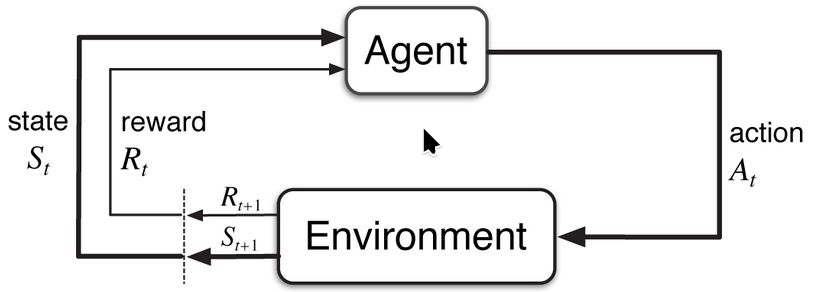
\includegraphics[width=0.8\linewidth]{agent_environment_loop.png}
    \caption[MDP agent-environment interaction]{Agent--environment interaction in a Markov Decision Process.}
    \label{fig:agent_environment}
\end{figure}



The goal of an agent is to learn an optimal strategy how to get best rewards(policy).  The core of this goal is a concept of the \textbf{action-value function}, or \textbf{Q-value}. The Q-value $Q(s,a)$ represents the expected return of action  $a$ in specific state $s$. Basically, it responds to the question:
\begin{quote}
    \emph{”How good is this action in this situation”}
\end{quote}

To reason about long-term consequences, reinforcement learning introduces the concept of \textbf{return}. The return $G_t$ is defined as the total accumulated reward an agent receives from time step $t$ onward. The return $G_t$ is defined as the discounted sum of future rewards:
$$G_t = R_{t+1} + \gamma R_{t+2} + \gamma^2 R_{t+3} + ... = \sum_{k=0}^{\infty} \gamma^k R_{t+k+1}$$
where $\gamma \in [0,1]$ is the \textbf{discount factor} that determines the present value of future rewards.


These values are related through the \textbf{Bellman principle}, which states that the value of a state or state--action pair depends on the immediate reward and the values of future states. In theory, this principle defines the optimal solution exactly. However, computing it directly requires full knowledge of the environment and repeated recursive updates, which is computationally infeasible for most real-world problems.  Approximation of Q-values happens from experience of an agent, and most methods of approximation are splited into 3 categories: \textbf{dynamic programming}, \textbf{Monte Carlo methods}, and \textbf{temporal-difference learning}. These approaches differ in how they use experience and feedback, and they form the foundation of the algorithms discussed in the following sections.


%%%%%%%%%%%%%%%%%%%%%%%%%%%%%%%%%%%%%%%%%%%%%%%%%%%%%%%%%%%%%%%%%%%%%%%%%%%%%%%
\section{Value Based Reinforcement Learning Algorithms}

\subsection{Dynamic Programming}

Dynamic Programming (DP) is a class of algorithms used to compute optimal value functions and policies when the \textbf{complete environment model is known}. For DP to be applicable, the problem must be formulated as a finite Markov Decision Process (MDP), and all states, actions, rewards, and transition dynamics $p(s', r \mid s, a)$ must be available.

Rather than solving the Bellman optimality equations directly, Dynamic Programming methods compute value functions iteratively using repeated updates of the form:

\[
\text{Old Value} \;\Rightarrow\; \text{Update Rule} \;\Rightarrow\; \text{New Value}
\]

These updates are applied repeatedly until the values converge.

Two main Dynamic Programming methods are commonly used:

\begin{itemize}

  \item \textbf{Policy Iteration}: alternates between policy evaluation and policy improvement. It typically converges in fewer iterations, but each iteration is computationally expensive.

  \item \textbf{Value Iteration}: combines policy evaluation and improvement into a single update. It requires more iterations, but each update is computationally cheaper.

\end{itemize}

Both methods are guaranteed to converge to the optimal policy and often converge quickly in small problems. However, Dynamic Programming is not very practical in real-world applications because it requires exact knowledge of the environment dynamics and becomes computationally intense for large state spaces.



\subsection{Monte Carlo Methods}

Monte Carlo methods require only experience. \cite{sutton}, without needing a model of the environment, its main difference from Dynamic Programing which requires full environment dynamics $p(s', r \mid s, a)$. 



Monte Carlo methods work only for \textbf{episodic tasks}, which means tasks that have an ending/finish.

  Sutton and Barto explicitly note that “to ensure that well-defined returns are available, here we define Monte Carlo methods only for episodic tasks” \cite{sutton}. Estimated values are being updated only at the end of the episode.

To make an estimation of the state -value function $v_\pi(s)$, an agent follows a policy $\pi$ and samples many episodes. Every time the agent is in state $s$, it records the return  $G_t$, which is a cumulative reward from that time step until the end of the episode, by averaging these returns, we get an estimated value of this state.  By the law of large numbers, sooner or later, this average would converge to the true expected value. 


\paragraph{Blackjack Example}  

%%%%%%%%%%%%
%  ADD figure of black jack gradient or not?
%%%%%%%%%%%%%%
As an example of MC, let's overview a classical casino game, “Blackjack”. Playing blackjack is naturally formulated as an episodic finite MDP. \cite{sutton}

Each game represents one episode, with rewards of $+1$, $0$, or $-1$ for a win, draw, or loss, respectively. All middle rewards are zero, and discounting is not required ($\gamma = 1$), meaning the return equals the final reward.

Each state is defined as a sum of the values of players' cards, if the dealer shows his cards, and if the agent has a usable ace. By iterating game episodes over and over under a fixed policy, MC would produce an accurate approximation of the state-value function. This would highlight an important advantage of Monte Carlo methods: while calculating the exact transition probabilities is difficult, the process of generating sample episodes to get probability approximation is straightforward.

Monte Carlo methods learn directly from experience and do not require a model of the environment. They do not bootstrap, meaning that value estimates are updated using complete returns rather than other estimates. MC methods are simple and intuitive, but they must wait until the end of an episode to update, which can result in high variance and slow learning. 


%\newpage
\subsection{Temporal Difference Learning}

Temporal-Difference learning or TD can be seen as a combination of Monte Carlo (MC) methods and Dynamic Programming (DP) \cite{sutton}. Like Monte Carlo methods, TD learning does not require a model of the environment and learns directly from experience. Like Dynamic Programming, TD methods update value estimates using other learned estimates, a process known as \textbf{bootstrapping}.

The key difference between TD and Monte Carlo methods is \textbf{when} updates are made. Monte Carlo methods must wait until the end of an episode to compute the full return and update values. In contrast, TD methods update estimates after each time step (it bootstraps), using the observed reward and the estimated value of the next state. This allows TD methods to learn \emph{online}, without waiting for the final outcome.




\paragraph{TD Prediction}

The simplest TD method is known as \textbf{TD(0)}, or one-step TD learning. The update rule for estimating the state-value function is given by:
\[
V(S_t) \leftarrow V(S_t) + \alpha \left[ R_{t+1} + \gamma V(S_{t+1}) - V(S_t) \right]
\]
where $\alpha$ is the learning rate and $\gamma$ is the discount factor.





The expression inside the brackets,
\[
\delta_t = R_{t+1} + \gamma V(S_{t+1}) - V(S_t),
\]
is called the \textbf{TD error}. It measures how different the current estimate is from a better estimate based on the next observed transition. This error signal plays a central role in almost all reinforcement learning algorithms.



Unlike Monte Carlo methods, TD methods do not require episodes to terminate and can therefore be applied to \textbf{continuing tasks}. This makes TD learning applicable to a wider range of real-world problems.






\paragraph{n-step TD and the MC--TD Connection}

TD learning can be generalized to \textbf{$n$-step TD methods}, which update values using $n$ future rewards:
\[
V(S_t) \leftarrow V(S_t) + \alpha \left[ G_{t:t+n} - V(S_t) \right]
\]
where
\[
G_{t:t+n} = R_{t+1} + \gamma R_{t+2} + \dots + \gamma^{n-1} R_{t+n} + \gamma^n V(S_{t+n}).
\]





These methods form a bridge between TD and Monte Carlo learning:
\begin{itemize}
\item $n = 1$ corresponds to TD(0),
\item $n \to \infty$ (or $n$ equal to episode length) corresponds to Monte Carlo learning.
\end{itemize}







\paragraph{Advantages of TD Learning}

TD methods offer several important advantages over Monte Carlo and Dynamic Programming approaches:
\begin{itemize}
\item Updates are performed after every step rather than once per episode.
\item TD methods can be applied to non-episodic (continuing) tasks.
\item Previously learned estimates can be reused immediately through bootstrapping.
\item In practice, TD methods often converge faster than Monte Carlo methods on stochastic problems \cite{sutton}.
\end{itemize}

These advantages are demonstrated in classical examples such as the random walk problem, where TD(0) is shown to achieve lower prediction error than constant-step-size Monte Carlo methods.





\paragraph{TD Control Methods}

TD learning can also be applied to the control problem by learning action-value functions $Q(s,a)$.

\textbf{Sarsa} is an on-policy TD control algorithm that updates values using the actual action taken by the agent:
\[
Q(S_t, A_t) \leftarrow Q(S_t, A_t) + \alpha \left[ R_{t+1} + \gamma Q(S_{t+1}, A_{t+1}) - Q(S_t, A_t) \right].
\]
Because Sarsa accounts for the agent’s exploration behavior, it often learns safer policies.




\textbf{Q-learning} is an off-policy TD control algorithm that directly learns the optimal action-value function:
\[
Q(S_t, A_t) \leftarrow Q(S_t, A_t) + \alpha \left[ R_{t+1} + \gamma \max_a Q(S_{t+1}, a) - Q(S_t, A_t) \right].
\]
Q-learning learns the optimal policy independently of the agent’s behavior, but its online performance can be unstable due to exploration.




\textbf{Expected Sarsa} replaces the maximum operator with an expectation over the policy, reducing variance and often improving performance in practice.





\section{From TD to DQN}
Within the TD framework, \textbf{Q-Learning} stands out as an off-policy algorithm that learns the optimal action-value function $Q^*(s, a)$ independently of the agent's behavior. The Q-learning update is:
$$Q(S_t, A_t) \leftarrow Q(S_t, A_t) + \alpha [R_{t+1} + \gamma \max_a Q(S_{t+1}, a) - Q(S_t, A_t)]$$

This specific equation is the direct mathematical ancestor of the **Deep Q-Network (DQN)**. By replacing the lookup table of $Q(s, a)$ with a deep neural network, DQN allowed RL to scale to high-dimensional environments like Atari games, which is a core focus of this project.


\subsection{Convolution Neural Networks and Deep Q Networks}

The main problem with Q-learning is that it does not scale well to large (or even medium) MDPs with many states and actions. For example, suppose you wanted to use Q-learning to train an agent to play Ms. Pac-Man (see Figure~\ref{fig:pacman}). There are about 150 pellets that Ms. Pac-Man can eat, each of which can be present or absent (i.e., already eaten). So, the number of possible states is greater than $2150 \approx 1045$. And if you add all the possible combinations of positions for all the ghosts and Ms. Pac-Man, the number of possible states becomes larger than the number of atoms in our planet, so there’s absolutely no way you can keep track of an estimate for every single Q-value. \cite{geron}

\begin{figure}[htbp]
\centering
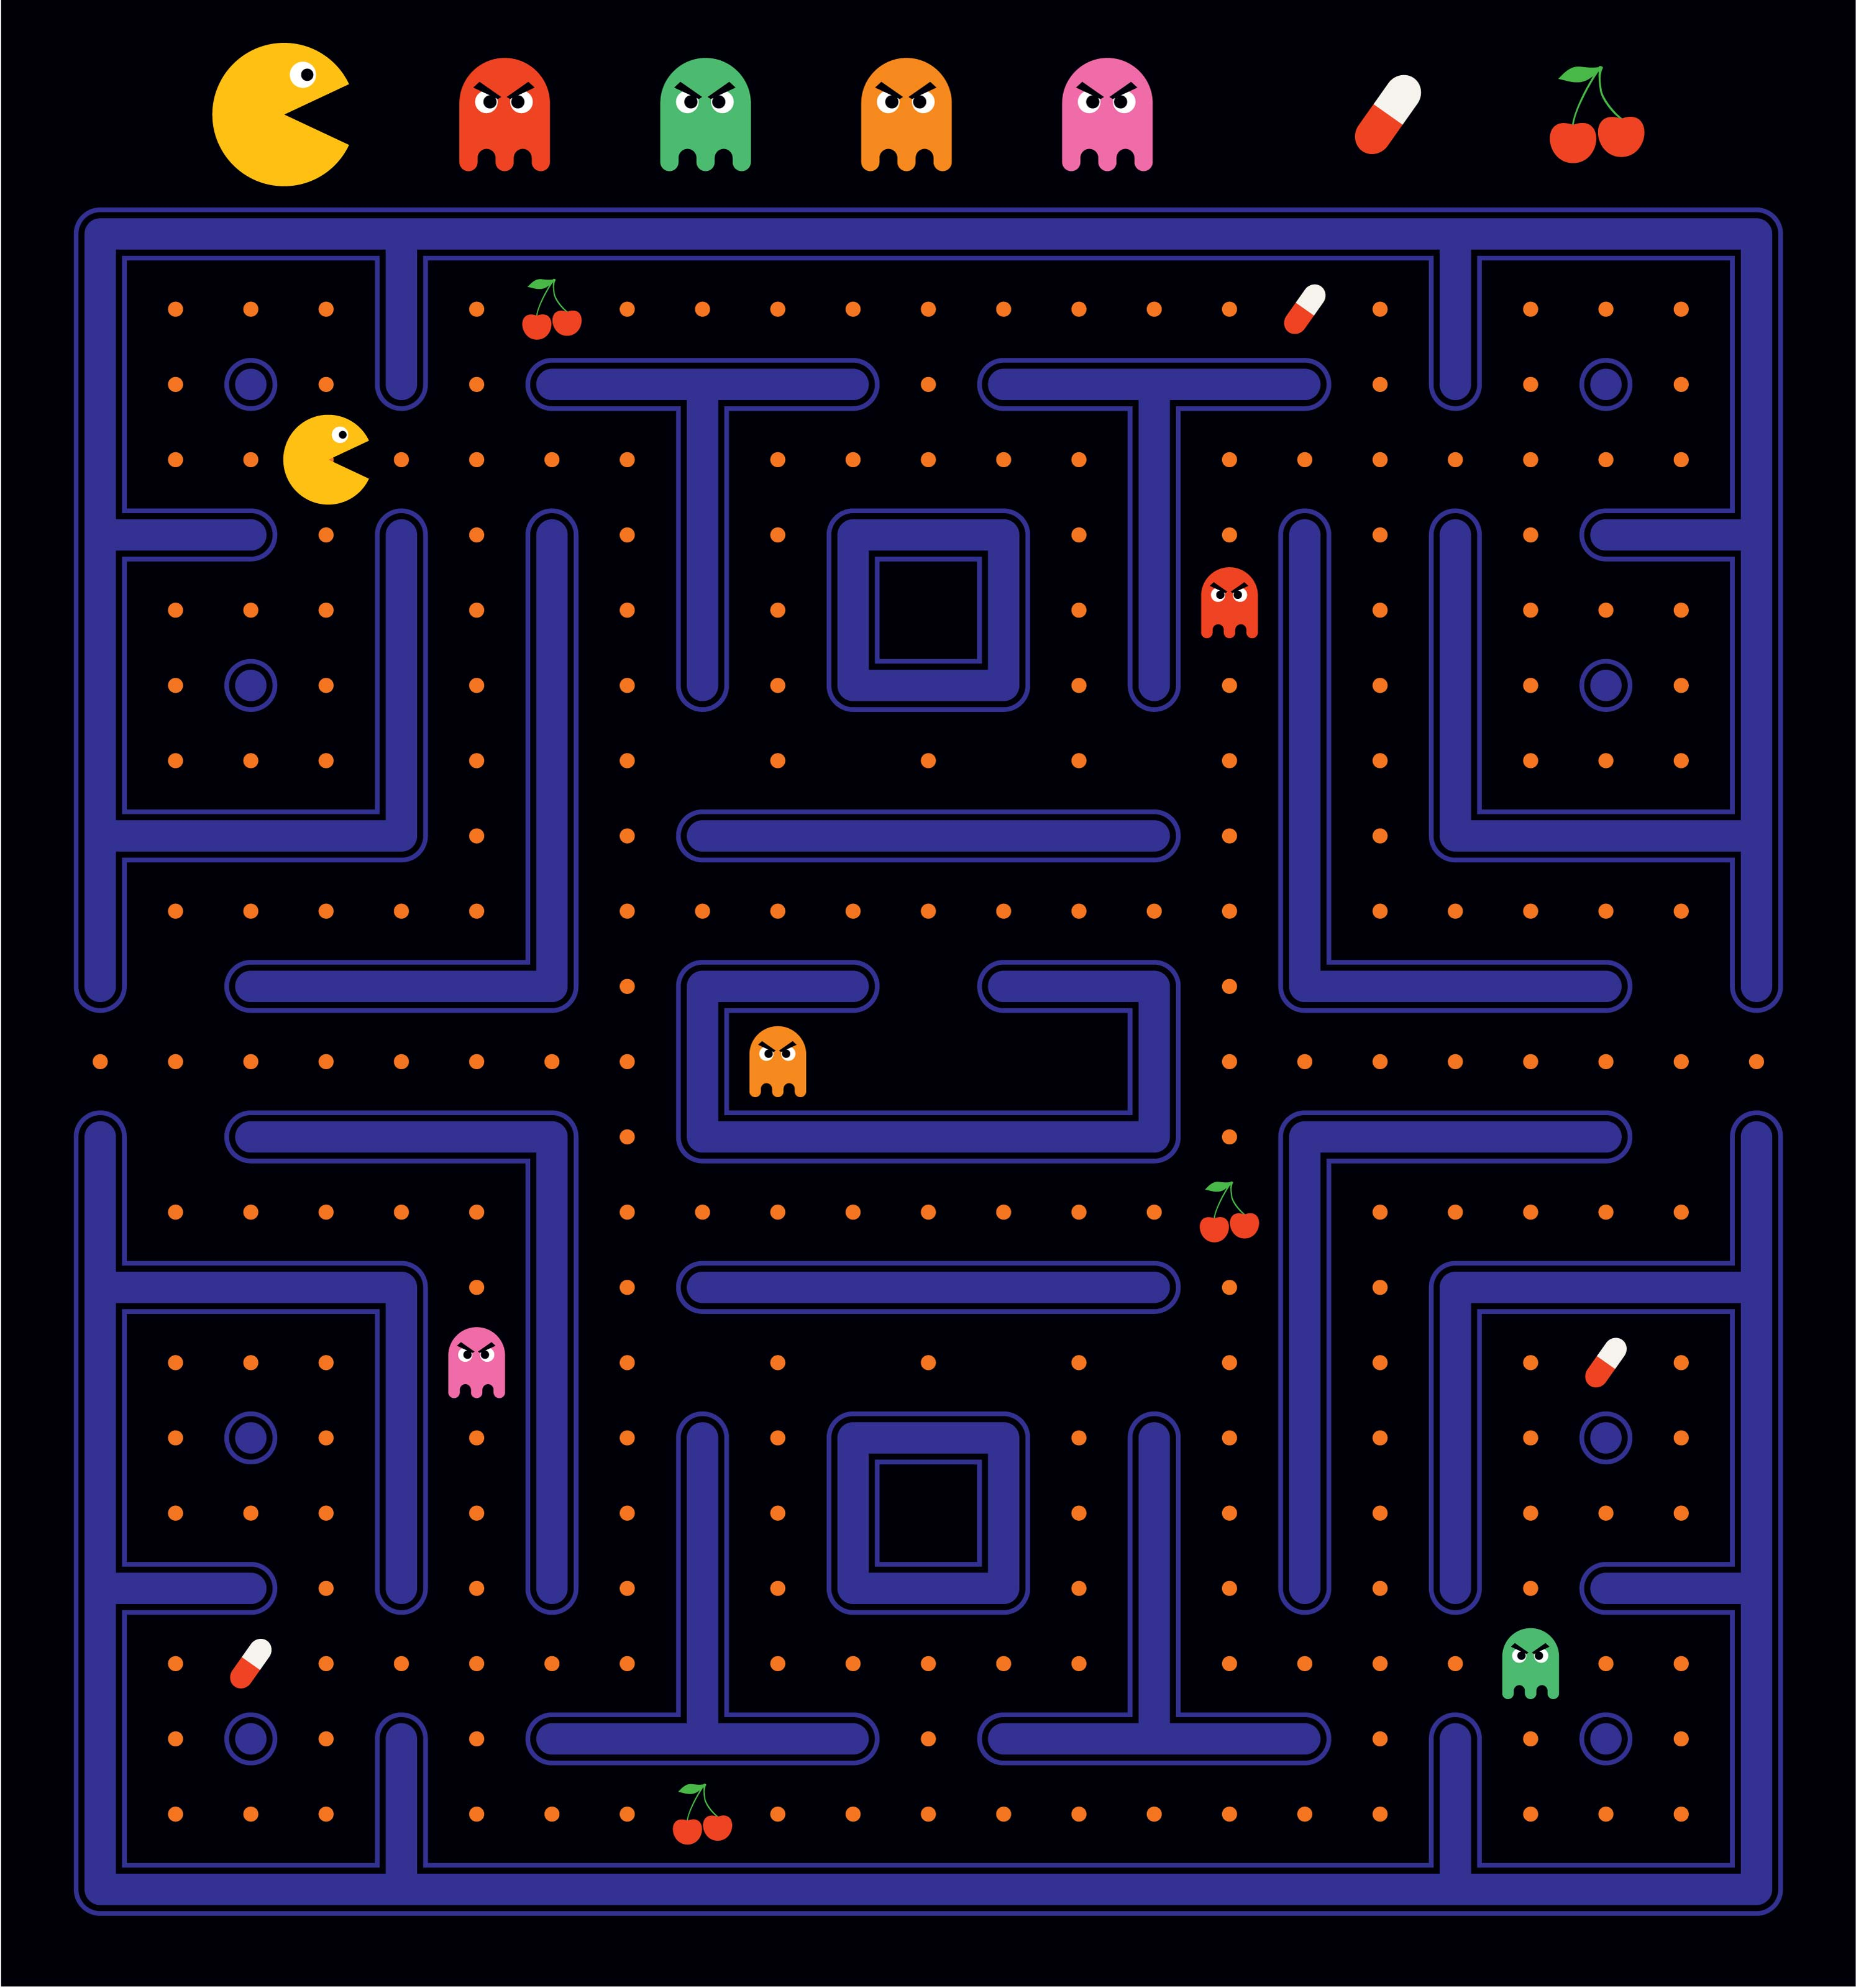
\includegraphics[width=0.5\linewidth]{pacman.jpg}
\caption[Pacman game example]{Pacman Game Example. Source: \cite{pacman_figure}}
\label{fig:pacman}
\end{figure}

The Solution is was suggested in 2013 by DeepMind when they published paper about DQN. \cite{mnih2015human}.
What they did is cobmined CNN with Q-learning and called it DQN.

\subsection{What is CNN}



Convolutional Neural Networks (CNNs) are a type of neural network designed specifically for data that comes in grid-like formats, such as images. Instead of treating every input value independently, a CNN works with small local regions of the image and learns filters that can detect useful patterns. These filters slide across the input, allowing the network to find the same pattern in different locations. This idea of local connections and shared weights is one of the core principles of CNNs, along with pooling and stacking multiple layers to build deeper feature representations \cite{lecun:hal-04206682}

\begin{figure}[htbp]
\centering
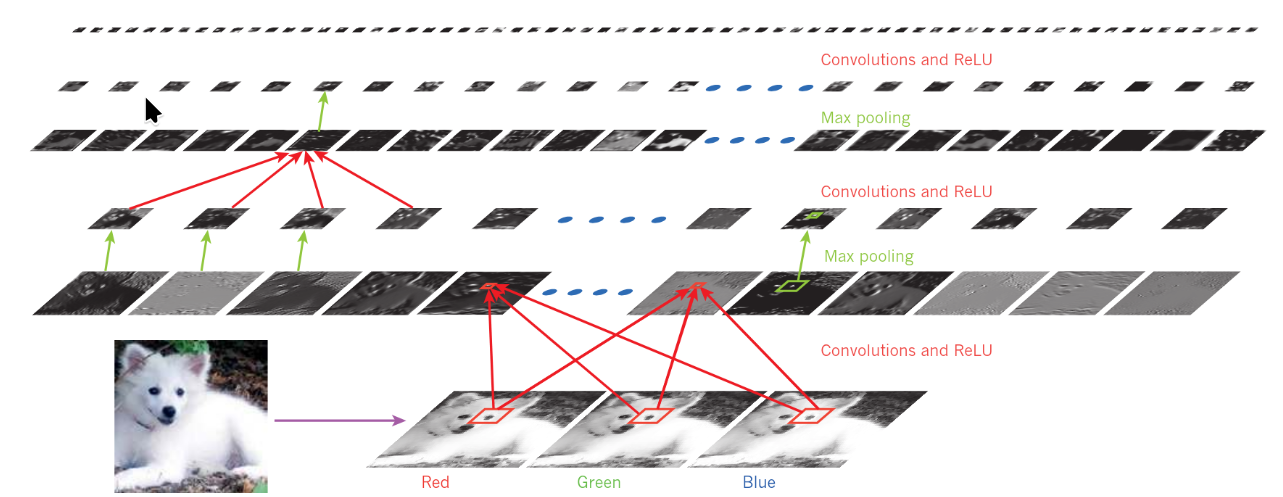
\includegraphics[width=1\linewidth]{cnn_1.png}
\caption[Inside a convolutional network]{Inside a convolutional network}
\label{fig:cnn_1}
\end{figure}

A typical CNN architecture, like the one shown in Figure~\ref{fig:cnn_1}, begins with convolutional layers that extract simple features such as edges or textures. These are followed by pooling layers, which reduce spatial resolution and make the representation more robust to small shifts in the input. By stacking several convolution–activation–pooling stages, the network gradually learns more abstract features: edges combine into motifs, motifs into shapes, and shapes into full objects. Finally, fully-connected layers interpret these features to produce the final output. This hierarchical processing makes CNNs especially powerful for visual tasks.

This ability to automatically extract meaningful features from raw images is exactly why CNNs became so important in reinforcement learning. Instead of trying to manually define state features—as classical Q-learning would require—a CNN can learn them directly from the raw game frames.

%\newpage
\subsection{DQN}

DeepMind were first who combined CNN and Q-learning algorithms, which made revolution in Reinforcment learning as their agent was first to learn directly from high-dimensional sensory input.

\begin{figure}[htbp]
\centering
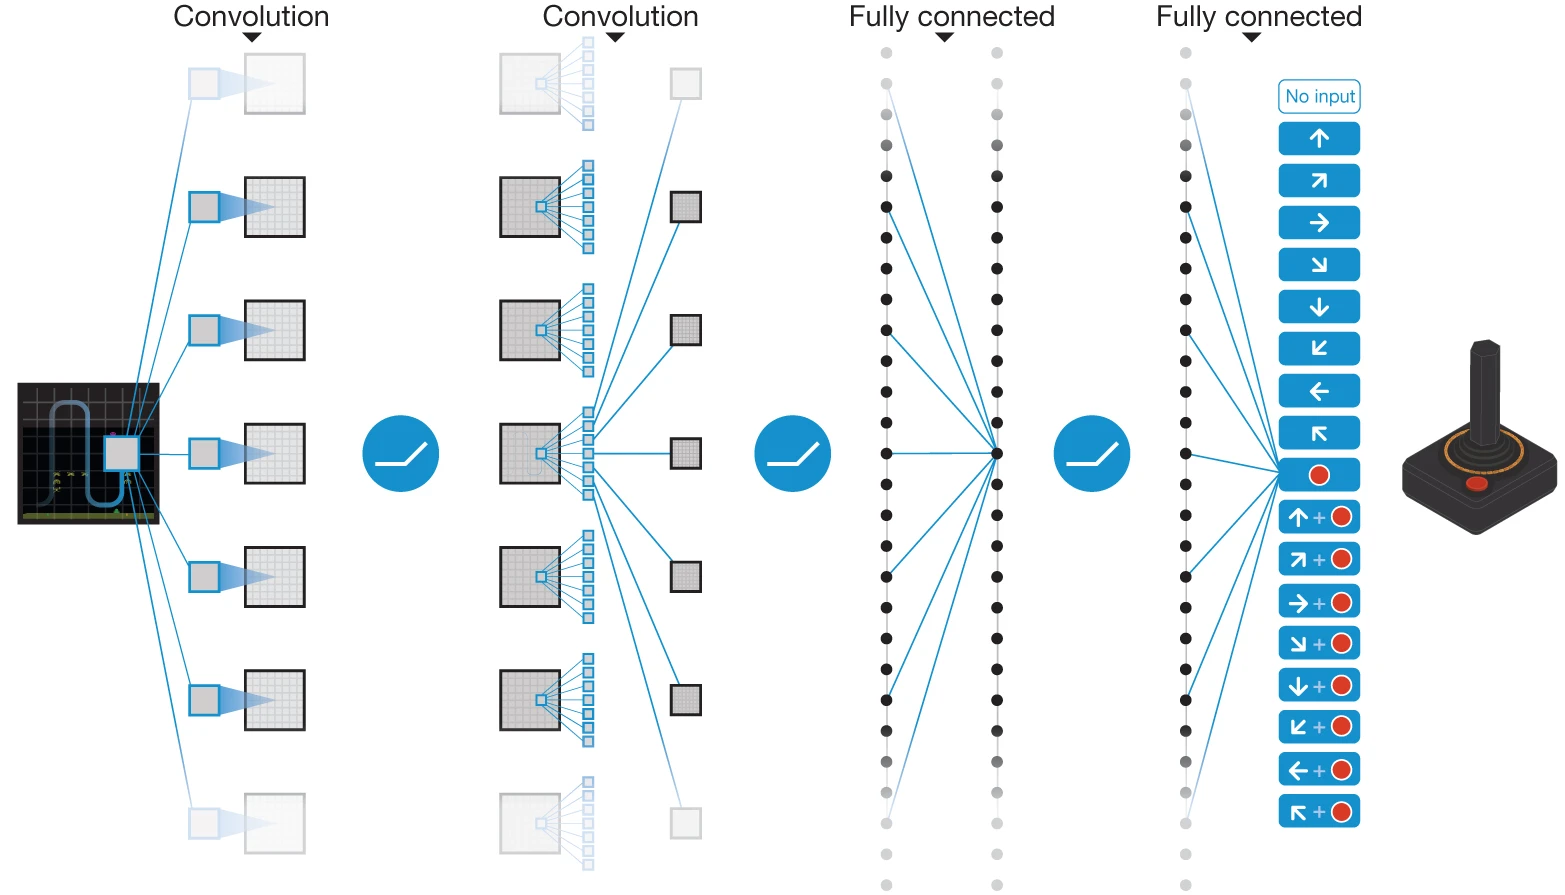
\includegraphics[width=1\linewidth]{dqn_1.png}
\caption[DQN architecture on Atari Breakout]{DQN Architecture on Atari Breakout \cite{mnih2015human}}
\label{fig:dqn_1}
\end{figure}

The CNN works by learning visual features automatically through repeated patterns - convolutional layers start with basic features like edges, then stack to detect increasingly complex objects. Starting from the left, raw game frames pass through these convolutional layers that extract visual features like edges and objects. They feed into fully connected layers that integrate spatial information, and Q-values for each action emerge on the right.
DQN also stabilized training with two key techniques: experience replay, which stores and randomly samples past experiences to break correlations, and a target network that updates slowly to provide stable learning targets. These innovations achieved human-level performance across 49 Atari games with a single algorithm.

Lets go through it in more details now.

In the original DeepMind system which is shown in Figure~\ref{fig:dqn_1} the input image (screenshot of the Atary game) consisted of 4 grayscale game frames staked together with dimensions of $84 \times 84$ pixels. This game agent knowledge not only of object positions but their velocity and motion directly without need to hand-craft this features. \cite{mnih2015human}

That input frames are passing to CNN network, first layer applies $32$ filters(kernels) of size $8 \times 8$ with stride size of 4, following by ReLu. Then on the third layer network applies 64 filters of size $4 \times 4$ with stride size of 2, following again by ReLu. The third layer applies another 64 filters but with cubic size of 3 this time and stride of 1. As a result we are getting mashed mozaic something which is flattened and fet into a fully–connected layer of 512 units, and finally into an output layer containing one
Q-value for each possible action in the game.

Training DQN uses a modified Q-learning loss function:
\[
L_i = \mathbb{E}_{(s,a,r,s')\sim U(D)}\left[ \big(r + \gamma \max_{a'} Q(s',a';\theta^{-})
- Q(s,a;\theta) \big)^2 \right],
\]
where $\theta$ are the network parameters and $\theta^{-}$ are the parameters of the
target network.


To make Q-learning stable with deep networks, DeepMind introduced two key innovations.
The first is \textit{experience replay}, which stores the agent’s past transitions and samples
them uniformly at random. This breaks the strong correlations between consecutive game
frames and allows the network to be trained using \textbf{\textit{minibatches}}, improving stability and data
efficiency. The second innovation is the use of a \textit{target network} whose parameters
$\theta^{-}$ are updated only every $C$ steps. This delays the bootstrapping updates and
prevents harmful feedback loops that would otherwise cause divergence when the network
tries to predict its own moving targets.

With these components combined, DQN became the first reinforcement learning agent to
achieve human-level performance across 49 Atari 2600 games using a single neural network
architecture and minimal prior knowledge. This result demonstrated that combining deep
learning with reinforcement learning enables agents to learn effective policies directly from
high-dimensional sensory input.


\section{Policy Gradients and Actor-Critic Methods}
All algorithms discussed above had something in common: they were value-based methods. They learned policy indirectly; for example, in DQN, the policy was derived from the values: we needed to calculate Q-values and then pick the largest one or do so at random. There is another group of algorithms that have a different strategy -- Policy Gradient.


These algorithms learn policy directly by parameterizing it; mathematicians use the symbol $\theta$ to denote it. If in previous algorithms, policy was marked as $\pi(s|a)$, and we needed an additional formula to predict best actions, in policy gradient policy with new parameter theta would be our formula of prediction and learning by itself, and it looks like this:
\[
\pi(a | s, \theta) = \text{Pr}\{A_t = a | S_t = s, \theta_t = \theta\}
\]

To be clearer, we have seen $\theta$ in formulas before, including in DQN. 

\[
L_i = \mathbb{E}_{(s,a,r,s')\sim U(D)}\left[ \big(r + \gamma \max_{a'} Q(s',a';\theta^{-})- Q(s,a;\theta) \big)^2\right],
\]


But it's different. In DQN, $\theta$ represented the network's weights that estimated the score (Q-value) of an action, whereas in Policy Gradient, theta represented the network's weights that directly determined the probability of an action. With Policy gradient, we don't need argmax anymore, because the network doesn't yield scores; it gives you the probability of each possible action, and we just sample from that distribution. 


By knowing the probabilities of each state in the environment, all that is needed for training is a slight nudge to parameter theta at each step, so the model can understand in which direction it should shift the probabilities. Unlike DQN, we don't need to know true values; all that matters is shifting theta based on the reward returned by the environment: higher reward -> higher shift in theta, to increase the probability of taking the same action next time.


It's important to note that to make the method work faster and more accurately, the critical part of this process is comparing of a reward agains a baseline; otherwise, if the agent were in a situation where actions draw a different reward, but all of them are positive, it would significantly slow down learning if there were no baseline. Policy gradient not just asks the question "did we get a reward?", but "did we get a better reward than usual?" instead. Baseline works by comparing the return ($G_t$) to a "Baseline" ($V(s)$). the formula also known as Policy Gradient Theorem:

\[
\theta_{t+1} = \theta_t + \alpha (G_t - b(S_t)) \nabla \ln \pi(A_t | S_t, \theta_t)
\]

Guarantees that we only need to compute the gradient of our own policy, which is fully known and differentiable, without needing to model the environment's complex dynamics.



\subsection{REINFORCE Algorithm}


The simplest implementation of Policy Gradient methods is REINFORCE, presented by Williams in 1988, which established a mathematical foundation for policy gradient methods \cite{Williams1988}. The name is an acronym for ``REward Increment = Nonnegative Factor $\times$ Offset Reinforcement $\times$ Characteristic Eligibility,'' which describes the form of the algorithm.


REINFORCE is a method used in reinforcement learning to improve how decisions are made. It learns by trying actions and then adjusting the chances of those actions based on the total reward received afterwards. Unlike other methods that estimate how good each action is, REINFORCE directly learns the best way to choose actions. This makes it useful for tasks where there are many possible actions or continuous choices and when it is hard to estimate the value of each action.


The core challenge REINFORCE addresses is that the environment is not differentiable. In reinforcement learning, an agent interacts with an environment that can be viewed as a black box: it processes an action and produces the next state and a reward. Since we cannot compute derivatives through the environment, we cannot backpropagate through it. The agent contains a neural network with learnable weights, and to update these weights, gradients are required. Because gradients through the environment are unavailable, we must find alternative ways to perform learning.


An intuitive analogy is a dog receiving treats. If an action leads to a good outcome, that action should be taken more often in the future. If one action produces a large reward, the probability distribution over actions should be adjusted so that this action becomes more likely while others become less likely. More generally, reward is used as a learning signal. When differentiation through the process that consumes network outputs is impossible, behavior is adjusted directly in the direction of reward. This is the core idea of REINFORCE.


Formally, consider a network facing an associative immediate-reinforcement learning task. Suppose that the learning algorithm for this network is such that at the end of each trial each parameter $w_{ij}$ in the network is incremented by an amount

\[
\Delta w_{ij} = \alpha_{ij}(r - b_{ij}) e_{ij},
\]

where $\alpha_{ij}$ is a learning rate factor, $b_{ij}$ is a reinforcement baseline, and

\[
e_{ij} = \frac{\partial \ln g_i}{\partial w_{ij}}
\]

is called the characteristic eligibility of $w_{ij}$. Suppose further that the reinforcement baseline $b_{ij}$ is conditionally independent of $y_i$, given $W$ and $x_i$, and the rate factor $\alpha_{ij}$ is nonnegative and depends at most on $w_{ij}$ and $t$. Any learning algorithm having this particular form will be called a REINFORCE algorithm \cite{williamsSimpleStatisticalGradientfollowing1992}.


In practice, REINFORCE operates on a policy $\pi_\theta(a|s)$ parameterized by $\theta$, which outputs an action given a state. The algorithm proceeds as follows. Initialize the policy parameters and step size $\alpha$. Then repeat:


\begin{enumerate}

\item Generate a full episode by following the policy:

$(s_0,a_0,r_1,s_1,\ldots,s_T)$.


\item For each timestep $t$, compute the discounted return:

\[
G_t = \sum_{k=0}^{T-t} \gamma^k r_{t+k+1}.
\]


\item Update parameters:

\[
\theta \leftarrow \theta + \alpha\, G_t \nabla_\theta \log \pi_\theta(a_t|s_t).
\]

\end{enumerate}


Actions are obtained by sampling from the policy distribution, typically produced via a softmax over network outputs. After sampling, the selected action is evaluated by computing its log-probability under the same policy. The loss is formed as:

\[
L = -G_t \log \pi_\theta(a_t|s_t).
\]

The negative sign is required because optimization minimizes loss while REINFORCE seeks to maximize expected return. REINFORCE uses reward as a surrogate gradient, allowing policy learning even when the environment is non-differentiable by directly increasing the probability of actions that lead to favorable outcomes.

REINFORCE algorithms are useful in their own right and, perhaps more importantly, may serve as a sound basis for developing other more effective reinforcement learning algorithms. One major advantage of the REINFORCE approach is that it represents a prescription for devising statistical gradient-following algorithms for reinforcement-learning networks of units that compute their random output in essentially any arbitrary fashion. Also, because it is a gradient-based approach, it integrates well with other gradient computation techniques such as backpropagation. The main disadvantages are the lack of a general convergence theory applicable to this class of algorithms and, as with all gradient algorithms, an apparent susceptibility to convergence to false optima \cite{williamsSimpleStatisticalGradientfollowing1992}.


\subsection{REINFORCE with Baseline}

One limitation of the basic REINFORCE algorithm is that it can exhibit unbounded behaviour \cite{Phansalkar1990optimization}. One improvement to address this is the introduction of a baseline. The policy gradient theorem can be generalized to include a comparison of the action value to an arbitrary baseline $b(s)$.

The baseline can be any function, even a random variable, as long as it does not vary with $a$; the equation remains valid because the subtracted quantity is zero. The update rule that we end up with is a new version of REINFORCE that includes a general baseline:
\[
\theta \leftarrow \theta + \alpha_\theta (G_t - b(S_t)) \nabla_\theta \log \pi(A_t|S_t,\theta).
\]

Because the baseline could be uniformly zero, this update is a strict generalization of REINFORCE. In general, the baseline leaves the expected value of the update unchanged, but it can have a large effect on its variance. This effect is demonstrated in Figure~\ref{fig:reinforce_baseline}, where adding a baseline significantly accelerates learning compared to plain REINFORCE.

\begin{figure}[htbp]
    \centering
    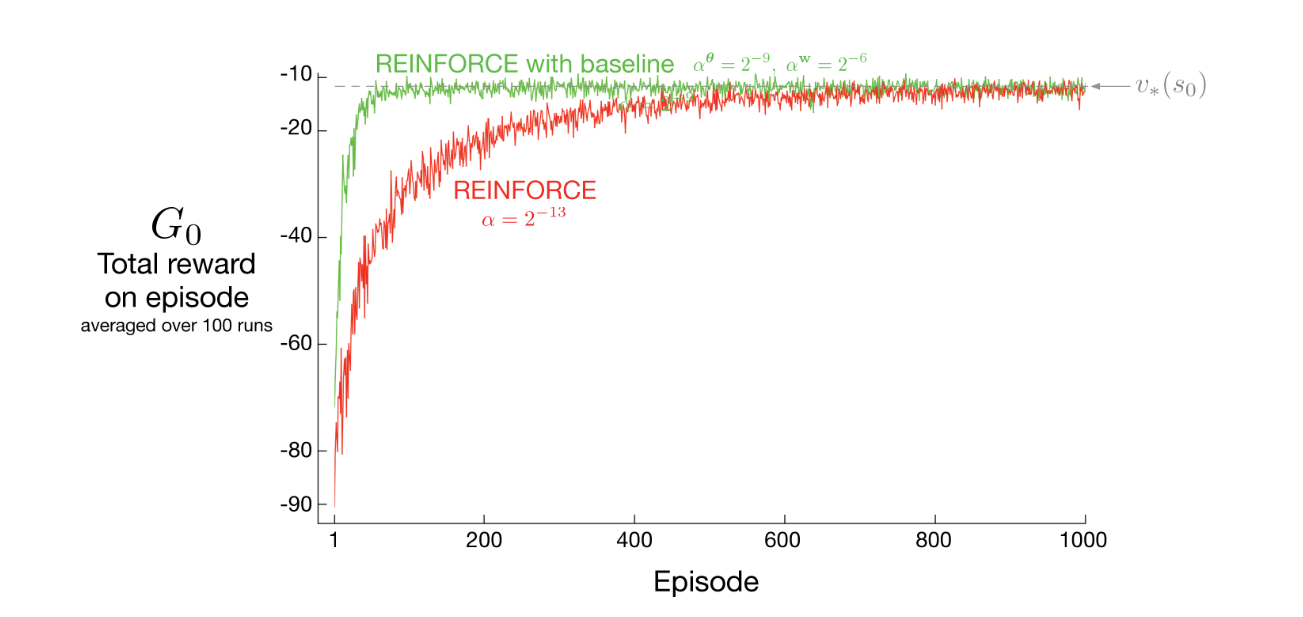
\includegraphics[width=0.8\linewidth]{ReinforceVSbaseline.png}
    \caption[REINFORCE with baseline comparison]{Adding a baseline to REINFORCE can make it learn much faster. The step size used for plain REINFORCE is that at which it performs best. Source: \cite{sutton}.}
    \label{fig:reinforce_baseline}
\end{figure}

For Markov decision processes, the baseline should vary with state. In some states all actions have high values and a high baseline is needed to differentiate the higher valued actions from the less highly valued ones; in other states all actions have low values and a low baseline is appropriate.

One natural choice for the baseline is an estimate of the state value, $\hat v(S_t,w)$, where $w \in \mathbb{R}^m$ is a weight vector learned by one of the methods presented previously. Because REINFORCE is a Monte Carlo method for learning the policy parameters $\theta$, it is natural to also use a Monte Carlo method to learn the state-value weights $w$.

% \newpage
\subsubsection{Episodic REINFORCE with Baseline}


Input: a differentiable policy parameterization $\pi(a|s,\theta)$


Input: a differentiable state-value function parameterization $\hat v(s,w)$


Algorithm parameters: step sizes $\alpha_\theta > 0$, $\alpha_w > 0$


Initialize policy parameter $\theta \in \mathbb{R}^{d'}$ and state-value weights $w \in \mathbb{R}^d$


For each episode:

\begin{enumerate}
\item Generate an episode $(S_0,A_0,R_1,\ldots,S_T)$ following $\pi(\cdot|\cdot,\theta)$
\item For each timestep $t = 0,1,\ldots,T-1$:
    \begin{enumerate}
    \item Compute return:
    \[
    G_t= \sum_{k=t+1}^{T} \gamma^{k-t-1} R_k
    \]
    \item Update state-value weights:
    \[
    w \leftarrow w + \alpha_w (G_t - \hat v(S_t,w)) \nabla_w \hat v(S_t,w)
    \]
    \item Update policy parameters:
    \[
    \theta \leftarrow \theta + \alpha_\theta (G_t - \hat v(S_t,w)) \nabla_\theta \log \pi(A_t|S_t,\theta)
    \]
    \end{enumerate}
\end{enumerate}

This algorithm has two step sizes, $\alpha_\theta$ and $\alpha_w$. Choosing the step size for the value function is relatively straightforward. It is less clear how to set the step size for the policy parameters, whose best value depends on the range of variation of rewards and on the policy parameterization \cite{sutton}.

Although the REINFORCE-with-baseline method learns both a policy and a state-value function, we do not consider it to be an actor–critic method because its state-value function is used only as a baseline, not as a critic. That is, it is not used for bootstrapping (updating the value estimate for a state from the estimated values of subsequent states), but only as a baseline for the state whose estimate is being updated \cite{sutton}.

% \newpage
\subsection{Actor -- Critic Methods}


Actor-Critic methods arise from policy gradient in the same way that TD learning emerged from Monte Carlo. Actor-Critic implements bootstrapping to solve the same waiting problem. In the original Policy Gradient (like Monte Carlo methods), we must wait until the full episode ends before updating our policy. This makes training slow and produces high-variance gradients. To mitigate this, instead of using actual returns, we estimate them.

In original policy gradient, the baseline b(s) could be any function—even just an average reward. But by making the baseline a learned value function ($b(s) = V(s)$), we effectively have two networks: one that picks actions (the policy $\pi$) called the Actor, and one that judges states (the value V) called the Critic. The actor 'performs'—deciding what action to take according to $\pi(a|s,\theta)$—while the critic 'criticizes' those actions, telling the actor whether a state is good or bad through $V(s,w)$. Note that these networks have separate parameters:$\theta$ for the actor and $W$ for the critic.

The critic enables bootstrapping. Instead of waiting for the full return $G_t$, we can estimate the advantage using the TD error:
\[
\delta_t = R_{t+1} + \gamma V(S_{t+1}) - V(S_t)
\]
This quantity estimates how much better the action taken was compared to the average action in that state.



To train both networks at the same time, we perform two updates at each time step:


Critic update: adjust w to make V(s) more accurate (same as TD learning from Section 2.5.3):

\[
w \leftarrow w + \alpha_w \delta_t \nabla V(S_t, w)
\]

Actor update: adjust $\theta$ using the critic's judgment:

\[
\theta \leftarrow \theta + \alpha_\theta \delta_t \nabla \ln \pi(A_t | S_t, \theta)
\]


Note that $\delta_t$ appears in both formulas—the critic's judgment guides everything, and this is how the two networks are connected.

\subsubsection{Advantages of Actor-Critic}

Actor-Critic methods combine the strengths of both value-based and policy-based approaches. Because they are built on policy gradients, they can learn stochastic policies, which is useful in environments requiring randomness (such as games with incomplete information). DQN, in contrast, is deterministic—it always selects the action with the maximum Q-value. Additionally, actor-critic methods can handle continuous action spaces (such as controlling a steering angle), whereas value-based methods require computing argmax over all possible actions, which is infeasible when actions are continuous.

Compared to pure policy gradient methods, actor-critic has lower variance because it uses TD estimates rather than waiting for full episode returns. This also means updates happen at every time step, enabling faster, online learning.

\subsection{Advantage Actor-Critic (A2C)}
\label{subsec:a2c}

Advantage Actor-Critic (A2C) is a synchronous variant of the Asynchronous Advantage Actor-Critic (A3C) method \citep{mnih2016a3c}, using the advantage function $A(s,a) = Q(s,a) - V(s)$ as the policy gradient signal to reduce variance while maintaining unbiased updates. Unlike A3C, which runs multiple actors in parallel threads with asynchronous gradient updates, A2C collects experience from all parallel environments synchronously before performing a single update, making it simpler to implement and reason about.
{\color{red} TODO: Expand this subsection with full description of A2C, advantage estimation, generalised advantage estimation (GAE)}

\subsection{Proximal Policy Optimisation (PPO)}
\label{subsec:ppo}

Proximal Policy Optimisation \citep{schulman2017ppo} is an actor-critic method that improves on A2C and REINFORCE by using a clipped surrogate objective to prevent excessively large policy updates, achieving stable training without the complexity of second-order trust-region methods (such as TRPO). PPO is currently one of the most widely used deep RL algorithms and serves as the primary actor-critic representative in the experiments of this thesis.
{\color{red} TODO: Expand this subsection with full description of the PPO clipped objective, generalised advantage estimation, epoch-level minibatch updates, and key hyperparameters.}



{\color{red}
\section{Experimental Frameworks and Tooling}
\label{sec:tooling}

\subsection{Gymnasium}
\label{subsec:gymnasium}
Gymnasium \citep{towers2024gymnasium} is a Python library providing a standardised interface for reinforcement learning environments. It is the maintained successor to OpenAI Gym and is now the de-facto standard for RL research and benchmarking. Gymnasium defines a consistent \texttt{reset}/\texttt{step}/\texttt{render} API that decouples algorithm implementations from environment details, making it straightforward to swap environments without changing training code. It ships with a wide range of reference environments, including the classic-control tasks (CartPole, Acrobot, LunarLander) used in Experiment~1 and, via the Arcade Learning Environment \citep{bellemare2013ale}, the Atari 2600 games used in Experiments~2 and~3. All environments in this thesis are instantiated through the Gymnasium API.

\subsection{Stable-Baselines3}
\label{subsec:sb3}
Stable-Baselines3 (SB3, v2.7.1) \citep{raffin2021sb3} is a set of reliable, well-tested PyTorch implementations of standard deep RL algorithms, including DQN, PPO, and A2C. It provides a consistent training API, built-in vectorised environments, evaluation utilities, and callback infrastructure. A key design goal of SB3 is reproducibility: all algorithms ship with carefully chosen default hyperparameters that are documented and stable across releases. This project uses SB3 exclusively for all algorithm implementations. Using a single, shared framework ensures that observed performance differences reflect genuine algorithmic properties rather than implementation quality or incidental hyperparameter choices.

\subsection{Stable-Baselines3 Contrib and Extensions}
\label{subsec:sb3contrib}
\texttt{sb3-contrib} is the official extension package for SB3, hosting algorithms that are functional but not yet part of the main stable release. Two algorithms used in Experiment~1 are sourced from this package: QR-DQN, a distributional variant of DQN that models the full return distribution rather than a scalar Q-value, and RecurrentPPO, a variant of PPO augmented with an LSTM layer to handle partial observability. Both are used with their \texttt{sb3-contrib} default hyperparameters under the same fair-comparison protocol as the main SB3 algorithms.

\subsection{Reproducibility Considerations}
\label{subsec:rliable}
Statistical evaluation in this thesis follows the \texttt{rliable} methodology of \citet{agarwal2021precipice}, which provides robust aggregate metrics (IQM, optimality gap, performance profiles, and probability of improvement) with stratified bootstrap confidence intervals. These metrics are more reliable than mean scores in the small-sample regime typical of RL research. The full evaluation protocol, including seeding strategy and score normalisation, is defined in Section~\ref{sec:eval-framework}.
}


\section{Evaluation Framework}
\label{sec:eval-framework}

This section defines what data are produced by reinforcement learning training, how evaluation scores are extracted from that data, and what metrics are used to compare algorithms throughout this thesis. Because this study uses a small set of $M \leq 3$ environments, \emph{per-environment} results are the primary evidence, and cross-environment aggregates are treated as descriptive summaries of the chosen tasks rather than universal generalisations \citep{agarwal2021precipice,patterson2024edrl}.

\paragraph{Seeding strategy.}
To ensure reproducibility while avoiding correlations induced by sequential seeding, all experimental runs were initialised from a single \emph{master seed}. Individual run seeds were deterministically derived using NumPy's \texttt{SeedSequence} spawning mechanism, which avoids linear relationships between seeds that may introduce inter-stream correlations in certain pseudorandom number generators \citep{matsumotoCommonDefectsInitialization2007}. All randomness sources (environment, NumPy, and PyTorch) were seeded using the derived run-specific seeds.

\subsection{Data Produced by RL Interaction}
\label{subsec:rl-data}

During training, at each time step $k$ the agent--environment interaction yields the transition tuple $(s_k,\,a_k,\,r_k,\,s_{k+1},\,d_k)$, where $s_k$ is the state, $a_k$ the action, $r_k$ the scalar reward, $s_{k+1}$ the next state, and $d_k\!\in\!\{0,1\}$ a terminal indicator. Algorithm comparisons are not made on training rewards directly, because training behaviour (exploration noise, replay buffer dynamics, on- vs off-policy sampling) is algorithm-dependent and not a stable measure of generalisation. Instead, a fixed \textbf{evaluation protocol} is used under which every algorithm is assessed identically.

\subsection{Evaluation Scores: Definitions and Notation}
\label{subsec:eval-scores}

An evaluation episode has an (environment-defined) length $H$, and the \textbf{episodic return} is $G = \sum_{k=0}^{H-1} r_k$. I report undiscounted $G$ throughout. Index conventions: $m$ over environments, $n$ over seeds, $t$ over evaluation checkpoints, $T$ the final checkpoint, $E$ the number of evaluation episodes. At each checkpoint $t$, the mean episodic return over $E$ episodes is:
\[
x_{m,n}(t)\;=\;\frac{1}{E}\sum_{e=1}^{E}G^{(e)}_{m,n}(t).
\]
These values form the \textbf{score matrix} $X(t)\in\mathbb{R}^{N\times M}$, with rows indexing seeds and columns indexing environments. All metrics below are computed from $X(T)$ at the final checkpoint.

\subsection{Uncertainty Quantification: Stratified Bootstrap}
\label{subsec:bootstrap}

Reinforcement learning exhibits high variance across independent training runs. To quantify statistical uncertainty, \textbf{95\% stratified bootstrap confidence intervals} are reported for all non-point-estimate metrics. For each environment $m$, seeds are resampled with replacement; the statistic is recomputed on each replicate and the 2.5\% and 97.5\% percentile bounds are taken. This procedure is recommended for the few-run regime \citep{agarwal2021precipice}.

\subsection{Per-Environment Metrics (Primary)}
\label{subsec:per-env-metrics}

Per-environment metrics operate on $\{x_{m,n}(t)\}_{n=1}^N$ for a fixed environment $m$:

\begin{itemize}
\item \textbf{Learning curve}: central tendency (mean or median over seeds) of $x_{m,n}(t)$ against training budget $t$, with pointwise uncertainty bands. Reveals learning dynamics that a single final number cannot capture.
\item \textbf{Final performance at fixed budget $T$}: central tendency of $\{x_{m,n}(T)\}$ with 95\% bootstrap CI. Answers ``how good is the agent after the same amount of experience?'' \citep{agarwal2021precipice}
\item \textbf{Sample efficiency}: normalised area under the learning curve, $\mathrm{AUC}_{m,n}=\sum_{j}x_{m,n}(t_j)(t_j-t_{j-1})/T$. Higher AUC indicates faster learning under the same budget.
\item \textbf{Reliability}: interquartile range (IQR) of $\{x_{m,n}(T)\}_n$ captures robustness across seeds \citep{chan2020reliability}.
\end{itemize}

\subsection{Cross-Environment Aggregate Metrics (Secondary)}
\label{subsec:cross-env-metrics}

Cross-environment metrics summarise the score matrix $X(T)$. With $M \leq 3$ environments, these are descriptive summaries rather than claims of general performance \citep{agarwal2021precipice,patterson2024edrl}:

\begin{itemize}
\item \textbf{Interquartile mean (IQM)}: pool all $MN$ values, trim the lowest and highest 25\%, average the middle 50\%. Robust to outliers and often yields tighter uncertainty in the few-run regime \citep{agarwal2021precipice}.
\item \textbf{Probability of improvement (POI)}: $P(A>B) = \frac{1}{M}\sum_m \Pr(x^A_{m,\cdot}>x^B_{m,\cdot})$. Interpretable probability that algorithm A outperforms B on a randomly chosen seed and environment.
\item \textbf{Performance profile}: fraction of runs $\hat{F}(\tau) = \frac{1}{MN}\sum_{m,n}\mathbb{I}[x_{m,n}(T)\ge\tau]$ at each threshold $\tau$. Visualises the full spectrum of outcomes.
\item \textbf{Optimality gap}: $\mathrm{Gap}(\tau) = \tau - \frac{1}{MN}\sum_{m,n}\min(x_{m,n}(T),\tau)$. Measures shortfall from a predefined target while clipping large outliers.
\end{itemize}


\section{Conclusion}


This chapter provided a high-level coverage of the basics of Reinforcement Learning, and should be sufficient for any reader to understand the idea of further implementations. It began with an overview of artificial intelligence and machine learning, then moved on to the core concepts of RL: MDPs, the Bellman equation, and exploration versus exploitation. Value-based methods came next—Dynamic Programming, Monte Carlo, TD Learning, and DQN. Finally, Policy, REINFORCE and Actor-Critic methods showed a different path: learning policy directly rather than through value estimation.
















